\chapter{Relational Data Model \& Relational Algebra} % Depth 0

\section{RDBMS}

\begin{itemize}
    \item Database Management System (DBMS) : a computer system for creating and maintaining databases
    \item Relational Database Management System (RDBMS) : databases which consists of \textit{tables} (relations)
\end{itemize}

\begin{figure}[H]
    \centering
    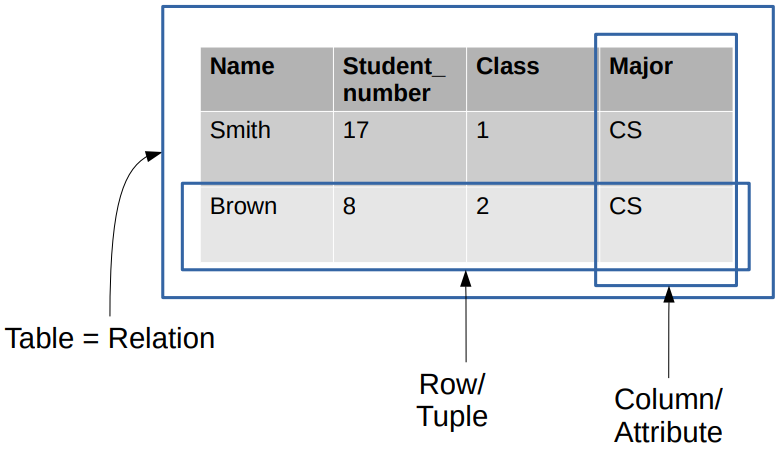
\includegraphics[width=0.6\textwidth,keepaspectratio]{RDBMS}
\end{figure}

\begin{Parallel}{0.47\textwidth}{0.47\textwidth}
\ParallelLText{
	\textgreen{\large{Pros}}
	\begin{itemize}
	    \item Ease of use due to abstraction (Logical/Physical independence)
	    \item Well known languages (SQL)
	    \item Reliability
	\end{itemize}
}

\ParallelRText{
	\textred{\large{Cons}}
	\begin{itemize}
	    \item Harder to obtain good performance, in particular in a distributed setting
	    \item Do not natively support very well some structures (Graph, Geographical data, Time-stamped data, ...)
	\end{itemize}
}
\ParallelPar
\end{Parallel}

\section{Relational Algebra}

Relational algebra is a set of mathematical rules and operators used to manipulate and query data in a relational database.

\subsection{Basic operators}

\begin{itemize}
    \item \textblue{Selection} $\sigma_{\text{(<selection condition>)}}(R)$ : used to denote the \textit{SELECT} operator. The \textit{selection condition} is a boolean expression specified on the attributes of relation \textit{R}
        \begin{itemize}
            \item It is \textit{commutative} : $\sigma_{(\text{<cond1>)}}(\sigma_{(\text{<cond2>})}(R)) = \sigma_{(\text{<cond2>})}(\sigma_{(\text{<cond1>})}(R))$
            \item A cascade of selections can be combined : $\sigma_{(\text{<cond1>})}(\sigma_{(\text{<cond2>})}(...(\sigma_{(\text{<condn>})}(R))...)) =$ \\$\sigma_{\text{(<cond1> \textbf{AND} <cond2> \textbf{AND} ... \textbf{AND} <condn>})}(R)$
            \item In Rel : $\sigma_{(\text{Age}=20)}$(Student) = $\{t \in \text{Student} \ | \ t.\text{Age}=19 \}$
            \item In SQL : SELECT * FROM Student WHERE Age=20
        \end{itemize}
    \item \textblue{Projection} $\pi_{\text{<attributes>}}$ : selects a subset of columns from a table. The operation \textbf{removes any duplicate tuples}, so the result is a set of distinct tuples, and hence a valid relation (known as \textbf{duplicate elimination})
        \begin{itemize}
            \item In Rel : $\pi_{\text{Age}}$(Student) = $\{ t[\text{Age}] \ | \ t \in \text{Student} \}$
            \item In SQL : SELECT DISTINCT Age FROM Student
        \end{itemize}
    \item \textblue{Union} $(\cup)$ : combines two tables and eliminated duplicate rows (of the same type)
    \item \textblue{Intersection} $(\cap)$ : returns only the rows (of the same type) that appears in both tables
    \item \textblue{Difference} $(-)$ : returns the rows of one table that do not appear in another tables (the types need to correspond). Contratry to Union and Intersection, it is \textbf{not commutative}.
    \item \textblue{Cartesian product} $(\times)$ : combines every row of one table with every row of another table, creating a new table with all possible combinations of rows. For example, you could use cartesian products to create a table that combines all possible pairs of products and customers.
    \item \textblue{Division} $(\div)$ : The division operation is used to retrieve tuples from one relation that are related to all tuples in another relation. Here is an example:
        \begin{itemize}
            \item R contains information about students (A) and the subjects they are enrolled in (B)
            \item S contains a list of subjects (B)
            \item R ÷ S will retrieve the students (tuples from R) who are enrolled in all subjects (tuples from S)
            \item R has the following tuples: ('John', 'Math') ('John', 'English') ('Mary', 'Math') ('Mary', 'Science')
            \item S has the following tuple: ('Math')
            \item R ÷ S will be: ('John') ('Mary')
        \end{itemize}
    \item \textblue{Assignment} $(\leftarrow)$ : used to split an expression in several intermediate steps.\\Example : $\pi_{\text{Name}}(\text{(Student)} - \pi_{\text{Name}}(\text{(Follows)}$ is equivalent to :
        \begin{itemize}
            \item $S' \leftarrow \pi_{\text{Name}}(\text{(Student)}$
            \item $F' \leftarrow \pi_{\text{Name}}(\text{(Student)}$
            \item $S' - F'$
        \end{itemize}
    \item \textblue{General rename} $(\rho)$ : used to rename the attributes in the intermediate relations.\\Example : $\rho_{(\text{Name} \rightarrow \text{Name1})}(\text{Follows})$
\end{itemize}

\subsection{Join operators}

The following "$\sigma_{A=B}(R_1 \times R_2)$" can be done using join operators as "$R_1 \bowtie_{A=B} R_2$"

\begin{itemize}
    \item \textblue{Theta join} $(\bowtie_{\theta})$ : combines tuples from two relations $R$ and $S$ based on a condition $\theta$ that involves attributes from both relations. The resulting relation contains all possible combinations of tuples from $R$ and $S$ \textit{that satisfy the condition}.
    \begin{itemize}
        \item \textblue{Equijoin} : special case of theta join where the condition is an equality comparison between attributes from the two relations. The resulting relation contains all possible combinations of tuples from R and S \textit{where the specified attributes are equal}.
    \end{itemize}
    \item \textblue{Natural join} $(\bowtie$ or $*)$ : performed between two relations with at least one common attribute. The join operation is done based on the common attribute(s) with the same name and domain in both relations. The resulting relation contains all possible combinations of tuples from $R$ and $S$ where the values of the common attributes are equal. Example :\\
    \begin{minipage}[t]{0.31\textwidth}
        \begin{center}
        \textgreen{Customer}\\
	    \begin{tabular}{|l|l|}
	    \hline 
	    Cid & Name \\ 
	    \hline 
	    \hline 
	    1 & Benjamin Bayer \\ 
	    \hline 
	    2 & Chung-cha Kim \\ 
	    \hline 
	    \end{tabular}
        \end{center}
    \end{minipage}
    \begin{minipage}[t]{0.31\textwidth}
        \begin{center}
        \textgreen{Buys}\\
	    \begin{tabular}{|l|l|}
	    \hline 
	    Cid & Pid \\ 
	    \hline 
	    \hline 
	    1 & A \\ 
	    \hline 
	    1 & B \\ 
	    \hline 
	    2 & B \\ 
	    \hline 
	    \end{tabular}
        \end{center}
    \end{minipage}
    \begin{minipage}[t]{0.31\textwidth}
        \begin{center}
        \textgreen{Product}\\
	    \begin{tabular}{|l|l|}
	    \hline 
	    Pid & Name \\ 
	    \hline 
	    \hline 
	    A & Cheese \\ 
	    \hline 
	    B & Milk \\ 
	    \hline 
	    \end{tabular}
        \end{center}
    \end{minipage}
    \begin{center}
    \textgreen{$\rho_{\text{Name} \rightarrow \text{CName}}(\text{Customer}) \bowtie \text{Buys} \bowtie \rho_{\text{Name} \rightarrow \text{PName}}(\text{Product})$}
    \begin{tabular}{|l|l|l|l|}
    \hline 
    Cid & CName & Pid & PName \\ 
    \hline
    \hline
    1 & Benjamin Bayer & A & Cheese \\ 
    \hline 
    1 & Benjamin Bayer & B & Milk \\ 
    \hline 
    2 & Chung-cha Kim & B & Milk \\ 
    \hline 
    \end{tabular} 
    \end{center}
    \newpage
    \item \textblue{Outer join} : includes all tuples from one or both participating relations, even if they do not satisfy the join condition. They are three types of outer joins :
    \begin{enumerate}
        \item \textblue{Left outer join} $(\leftouterjoin)$ : join that inserts \textit{NULL} for tuples missing in the second relation.
        \item \textblue{Right outer join} $(\rightouterjoin)$ : join that inserts \textit{NULL} for tuples missing in the first relation.
        \item \textblue{Full outer join} $(\fullouterjoin)$ : join that inserts \textit{NULL} for tuples missing in the other relation.
    \end{enumerate}
    \begin{minipage}[t]{0.48\textwidth}
        \begin{center}
        \textgreen{Customer}\\
	    \begin{tabular}{|l|l|}
	    \hline 
	    Cid & Name \\ 
        \hline
        \hline
	    1 & Benjamin Bayer \\ 
	    \hline 
	    2 & Chung-cha Kim \\ 
	    \hline 
	    3 & Barbara Benson \\ 
	    \hline 
	    \end{tabular}
        \end{center}
    \end{minipage}
    \begin{minipage}[t]{0.45\textwidth}
        \begin{center}
        \textgreen{Buys}\\
	    \begin{tabular}{|l|l|}
	    \hline 
	    Cid & Pid \\ 
        \hline
        \hline
	    1 & A \\ 
	    \hline 
	    1 & B \\ 
	    \hline 
	    2 & B \\ 
	    \hline 
	    4 & A \\ 
	    \hline 
	    \end{tabular}
        \end{center}
    \end{minipage}
    
    
    \smallskip
    \begin{minipage}[t]{0.3\textwidth}
        \begin{center}
        \textgreen{Customer $\leftouterjoin$ Buys}\\
        \begin{tabular}{|l|l|l|}
        \hline
        Cid & Name & Pid \\
        \hline
        \hline
        1 & B. Bayer & A \\
        \hline
        1 & B. Bayer & B \\
        \hline
        2 & C. Kim & B \\
        \hline
        3 & B. Benson & NULL \\
        \hline
        \end{tabular}
        \end{center}
    \end{minipage}
    \begin{minipage}[t]{0.3\textwidth}
        \begin{center}
        \textgreen{Customer $\fullouterjoin$ Buys}\\
        \begin{tabular}{|l|l|l|}
        \hline
        Cid & Name & Pid \\
        \hline
        \hline
        1 & B. Bayer & A \\
        \hline
        1 & B. Bayer & B \\
        \hline
        2 & C. Kim & B \\
        \hline
        3 & B. Benson & NULL \\
        \hline
        4 & NULL & A \\
        \hline
        \end{tabular}
        \end{center}
    \end{minipage}
    \begin{minipage}[t]{0.3\textwidth}
        \begin{center}
        \textgreen{Customer $\rightouterjoin$ Buys}\\
        \begin{tabular}{|l|l|l|}
        \hline
        Cid & Name & Pid \\
        \hline
        \hline
        1 & B. Bayer & A \\
        \hline
        1 & B. Bayer & B \\
        \hline
        2 & C. Kim & B \\
        \hline
        4 & NULL & A \\
        \hline
        \end{tabular}
        \end{center}
    \end{minipage}
\end{itemize}

\chapter{The Relational Model \& Integrity Constraints}

\section{Domain constraints}

Every attribute has a domain, only values within the domain are allowed (i.e. \textit{VARCHAR, INT, CHAR, DATE}) and it is possible to explicitly allow/disallow \textit{NULL} for each attribute. It's also possible to restrict the range of allowed values, and define new types (based on existing types or enumerations).

Example :

\begin{minted}{sql}
CREATE DOMAIN SSN_TYPE AS CHAR(9):
CREATE DOMAIN D_NUM AS INT
    CHECK (Dnumber > 0 AND Dnumber < 21);
CREATE TYPE GENDER_TYPE AS ENUM ('M', 'F', 'N');

CREATE TABLE DEPARTMENT (
    Dname VARCHAR(15) NOT NULL,
    Dnumber D_NUM NOT NULL,
    Mgr_ssn SSN_TYPE NOT NULL,
    Mgr_start_date DATE );
\end{minted}

\section{Key constraints}

\begin{itemize}
    \item \textblue{Superkey} : a set of one or more attributes that can uniquely identify a tuple (row) in a table. In other words, a superkey is a combination of one or more attributes that can garantee the uniqueness of each tuple in a table.
    \item \textblue{Key} : a minimal superkey; a superkey that has no other superkey as its subset.
    \item If a relation has multiple keys, all these keys are also called \textblue{candidate keys}. In database design it is common to indicate one the candidate keys as the \textblue{primary key}. The other candidate keys are \textblue{unique keys}.
    \item \textblue{Foreign key} : a field or combination of gields in one table that refers to the primary key of another table. It establish a relationship between two tables by ensuring referential integrity (meaning that data in one table is consistent with data in another table).
\end{itemize}

\section{Transaction}

Set of database operations that is executed in a manner that is \textblue{ACID} :
\begin{itemize}
    \item \textblue{A}tomic : After executing the transaction, all operations in the transaction have been executed, or none.
    \item \textblue{C}onsistent : After the transaction, all constraints are satisfied. Constraints are checked after all operations in the transaction have been executed, and all operations in the transaction are rejected if the result violates constraints.
    \item \textblue{I}solated : If multiple transactions are initiated at the same time, the database system will ensure that they are executed sequentially, such that one transaction is executed entirely before the other one is executed.
    \item \textblue{D}urable : If the database has indicated to a user program that it has finished executing a transaction, its results should be durable : the database remains in the correct state even in case of a power failure.
\end{itemize}

\chapter{Conceptual Modeling using Diagrams}

\section{Designing a Relational Database}

\subsection{Conceptual vs Physical Design}

\begin{minipage}[t]{0.48\textwidth}
\paragraph*{Conceptual design}
Visualization of the information that we conceptually plan to store; the decision how to link the tables to each other in the relational database is not made yet.
\end{minipage}
\hfill
\begin{minipage}[t]{0.48\textwidth}
\paragraph*{Physical design}
Every attribute in the relational database is listed, lines correspond exactly to foreign key relationships.
\end{minipage}

\begin{minipage}{0.48\textwidth}
\begin{figure}[H]
    \centering
    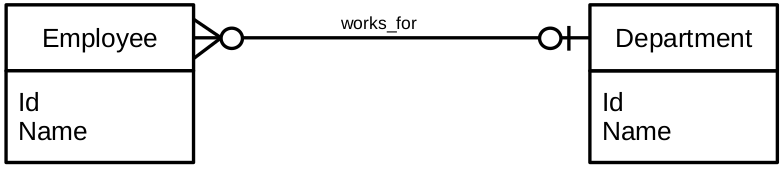
\includegraphics[width=\textwidth,keepaspectratio]{conceptual_d}
\end{figure}
\end{minipage}
\hfill
\begin{minipage}{0.48\textwidth}
\begin{figure}[H]
    \centering
    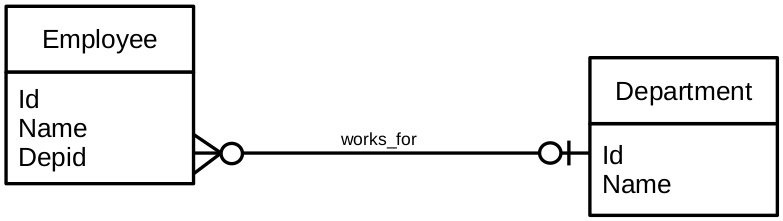
\includegraphics[width=\textwidth,keepaspectratio]{physical_d}
\end{figure}
\end{minipage}

\subsection{Different Types of Diagrams}

\begin{minipage}[t]{0.48\textwidth}
\paragraph*{Er-Chen}
\begin{itemize}
    \item Boxes for entities
    \item Diamonds for relationship
\end{itemize}
\end{minipage}
\hfill
\begin{minipage}[t]{0.48\textwidth}
\paragraph*{Crow's foot}
\begin{itemize}
    \item Boxes for entities
    \item Lines for relationship
\end{itemize}
\end{minipage}

\begin{minipage}{0.48\textwidth}
\begin{figure}[H]
    \centering
    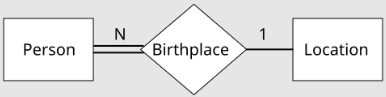
\includegraphics[width=\textwidth,keepaspectratio]{er-chen_example}
\end{figure}
\end{minipage}
\hfill
\begin{minipage}{0.48\textwidth}
\begin{figure}[H]
    \centering
    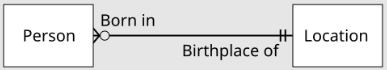
\includegraphics[width=\textwidth,keepaspectratio]{crow_foot_example}
\end{figure}
\end{minipage}

%
\begin{minipage}[t]{0.48\textwidth}
\paragraph*{Object Role}
\begin{itemize}
    \item Circles for objects
    \item Boxes for objects
\end{itemize}
\end{minipage}
\hfill
\begin{minipage}[t]{0.48\textwidth}
\paragraph*{UML}
\begin{itemize}
    \item Boxes for classes
    \item Lines for associations
\end{itemize}
\end{minipage}

\begin{minipage}{0.48\textwidth}
\begin{figure}[H]
    \centering
    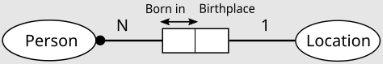
\includegraphics[width=\textwidth,keepaspectratio]{object_role_example}
\end{figure}
\end{minipage}
\hfill
\begin{minipage}{0.48\textwidth}
\begin{figure}[H]
    \centering
    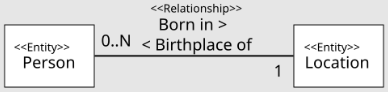
\includegraphics[width=\textwidth,keepaspectratio]{uml_example}
\end{figure}
\end{minipage}

\newpage
\subsection{Relationship multiplicities}

\subsubsection{1:1 multiplicity}

Refers to the number of occurrences of a relationship between two tables in database design. When a 1:1 multiplicity is not mandatory, it means that the relationship is optinal and not every record in one table need to be related to a record in the other table.

\begin{minipage}{0.45\textwidth}
\begin{figure}[H]
    \centering
    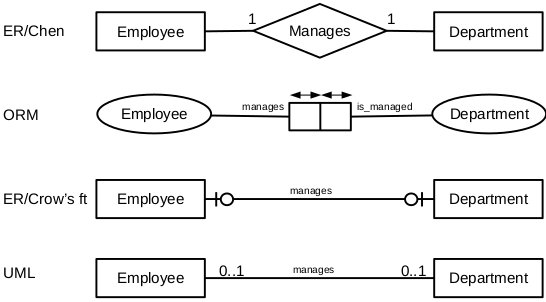
\includegraphics[width=0.8\textwidth,keepaspectratio]{1_1_mult_1}
\end{figure}
\end{minipage}
\hfill
\begin{minipage}{0.45\textwidth}
\begin{figure}[H]
    \centering
    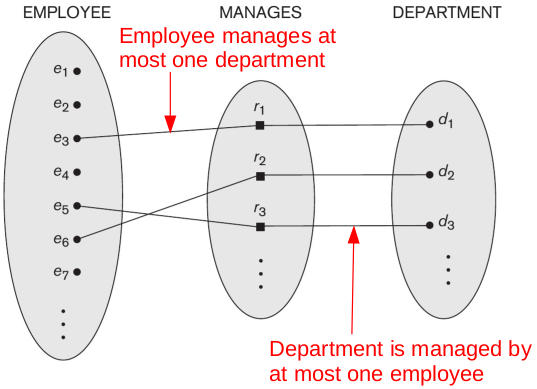
\includegraphics[width=0.7\textwidth,keepaspectratio]{1_1_mult_2}
\end{figure}
\end{minipage}


\subsubsection{M:N multiplicity}

Refers to a many-to-many relationship between two tables. When a M:N multiplicity is not mandatory, it means that the relationship between the tables is optinal, and not every record in one table needs to be related to a record in the other table.

\begin{minipage}{0.45\textwidth}
\begin{figure}[H]
    \centering
    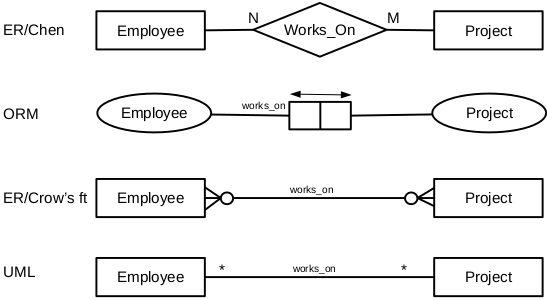
\includegraphics[width=0.8\textwidth,keepaspectratio]{M_N_mult_1}
\end{figure}
\end{minipage}
\hfill
\begin{minipage}{0.45\textwidth}
\begin{figure}[H]
    \centering
    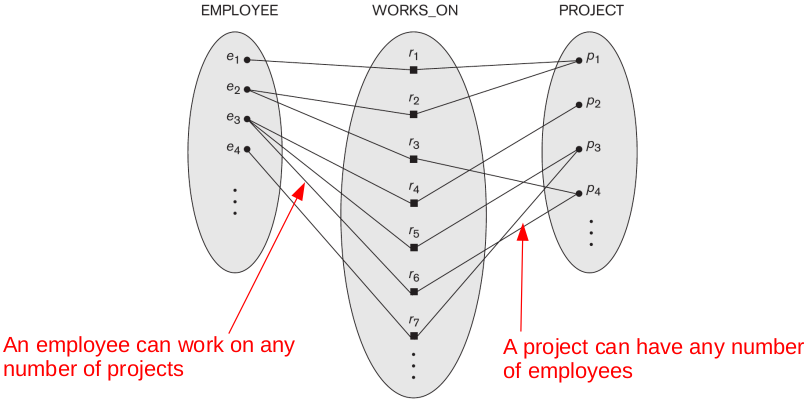
\includegraphics[width=0.8\textwidth,keepaspectratio]{M_N_mult_2}
\end{figure}
\end{minipage}

\subsubsection{1:N multiplicity}

Refers to a one-to-many relationship between two tables

\begin{minipage}{0.45\textwidth}
\begin{figure}[H]
    \centering
    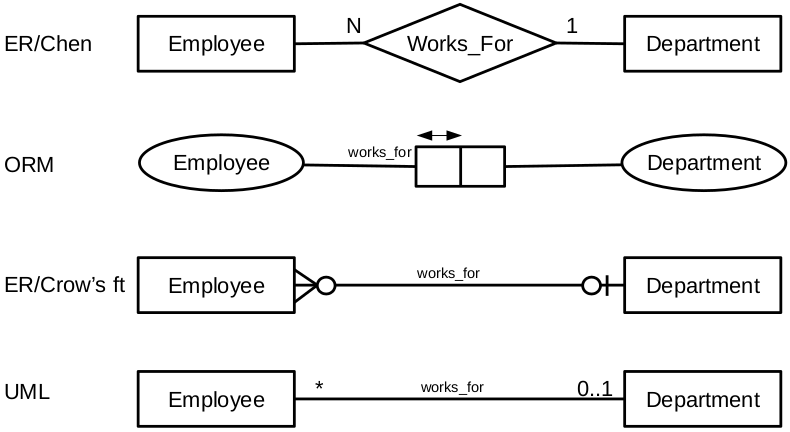
\includegraphics[width=0.8\textwidth,keepaspectratio]{1_N_mult_2}
\end{figure}
\end{minipage}
\hfill
\begin{minipage}{0.45\textwidth}
\begin{figure}[H]
    \centering
    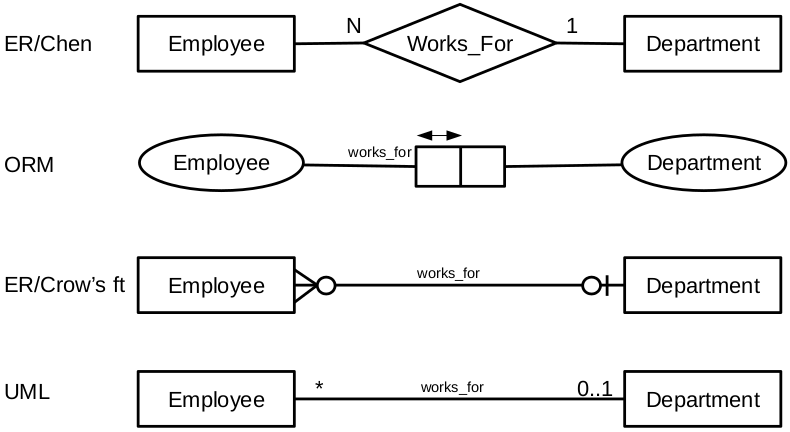
\includegraphics[width=0.8\textwidth,keepaspectratio]{1_N_mult_1}
\end{figure}
\end{minipage}
